% Gute Quelle:
% http://winfwiki.wi-fom.de/index.php/Wertsch%C3%B6pfungsnetzwerke_und_Industrie_4.0

% Masterarbeit Alex
% https://www.yumpu.com/de/document/view/21142108/schriftliche-ausarbeitung-alexander-willner-masterarbeit/5

% https://de.slideshare.net/KarlIsenberg/container-orchestration-wars

\chapter{State of the art}\label{chapter:state-of-the-art}
This chapter will give an overview into the background and concepts of this thesis.
In the first section the Internet of Things an related subtopics like Smart Factories and Smart Cities are considered.
Cyber Physical Systems, which are important for the development of Smart Factories are also covered in this section.
Virtualization in general is the main topic of the second section.
First we dive into the area of Virtual Machines, followed by Container Virtualization.
Both are related to each other and sharing some basic ideas.
Container Orchestration as an own subsection show some possibilities of Container Virtualization.
The last subsection Network Function Virtualization concludes with an introduction into the virtualization of network node functions to create communication services.


\section{Internet of Things}
The \ac{IoT} has been a subject of great media- and economically growth in the recent years.
In the year 2008 the number of devices which are connected to the Internet was higher than the human population.\cite[cf.]{Eva11}
Cisco Internet Business Solutions Group predicted that the number will grow up to 50 billion in 2020, this equates to around 6 devices per person.\cite[cf.]{Eva11}
Most of today\'s interactions are \ac{H2H} or \ac{H2M} communication.
The \ac{IoT} on the other hand aim for the \ac{M2M} communication.
This allows every physical devices to be interconnected and to communicate with each other.
These devices are also called "Smart Devices".
Creating a network where all physical objects and people are connected via software is one primary goal of the \ac{IoT}.\cite[cf.]{Rui2015}\cite[cf.]{Kra13}
When objects are able to capture and monitor their environment, a network can perceive external stimuli and respond to them.\cite[cf.][p. 40]{Itu11}
Therefore a new dimension of information and communication technology will be created, where users have access to everything at any time, everywhere.
In addition to smart devices, subcategories are also emerging from the \ac{IoT} which, in addition to the physical devices, also describe technologies such as protocols and infrastructures.
The "`Smart Home"' has been a prominent topic in media and business for many years.
Smart City or Industrie 4.0 are also becoming established and are increasingly popular.
But the Internet started with the appearance of bar codes and \ac{RFID} chips.\cite[cf.]{Kra13}
The second step, which is more or less the current situation, sensors, physical devices, technical devices, data and software are connected to each other.\cite[cf.]{Kra13}
This was achieved, in particular, by cloud computing, which provides the highly efficient memory and computing power that is indispensable for such networks.\cite[cf.]{Rui2015}
The next step could be a "`Cognitive Internet of Things"', which enables easier object and data reuse across application areas, for example through interoperable solutions, high-speed Internet connections and a semantic information distribution.\cite[cf.]{Kra13}
Just as the omnipresent information processing in everyday life, also known as "`Ubiquitous Computing"', which was first mentioned in the "`The Computer for the 21st Century"'\cite[cf.]{Wei91} by Marks Weiser, it will take some time until it is ubiquitous.


\subsection{Industry 4.0 and Smart Factories}
The industry as an changing environment is currently in the state of the so called "fourth industrial revolution".
The first industrial revolution was driven by steam powered machines.
Mass production and division of labor was the primary improvement of the second industrial revolution, whereas the third revolution was characterized by using electronics and the integration of \ac{IT} into manufacturing processes.\cite[cf.][p. 1]{Lom:2016}
In the recent years the size, cost and power consumption of chipsets are reduced which made it possible to embed sensors into devices and machines much easier and cheaper.\cite[cf.][p. 1]{Brito2016}
The Industry 4.0 is the fourth step in this evolution and was first mentioned with the German term "Industrie 4.0" at the Hannover Fair in 2011.\cite[cf.][p. 1]{Lom:2016}
"Industrie 4.0 is a collective term for technologies and concepts of value chain organization."\cite[cf.][p. 11]{Her2015}

Significantly higher productivity, efficiency, and self-managing production processes where everything from machines up to goods can communicate and cooperate with each other directly are the visions of the Industry 4.0.\cite[cf.]{Lyd2016}
It also aims for an intelligent connection between different companies and units.
Autonomous production and logistics processes creating a real-time lean manufacturing ecosystem that is more efficient and flexible.\cite[cf.]{Lyd2016}
"This will facilitate smart value-creation chains that include all of the life-cycle phases of the product from the initial product idea, development, production, use, and maintenance to recycling."\cite{Lyd2016}
At the end, the system can use customer wishes in every step in the process to be flexible and responsive.\cite[cf.]{Lyd2016}

\taburulecolor{ob_dark_gray}
\begin{table}[htpb]
  \centering
    \begin{tabular}{| r | c c c c |}
      \rowcolor{ob_orange}
      \hline
                            & Cyber-Physical & Internet  & Internet    & Smart Factory \\
      \rowcolor{ob_orange}
                            & Systems        & of Things & of Services &  \\
      \hline
      Interoperability      & X        & X        & X          & X    \\
      Virtualization        & X        & -        & -          & X    \\
      Decentralization      & X        & -        & -          & X    \\
      Real-Time Capability  & -        & -        & -          & X    \\
      Service Orientation   & -        & -        & X          & -    \\
      Modularity            & -        & -        & X          & -    \\
      \hline
    \end{tabular}
  \caption[Design principles of each Industry 4.0 component]{Design principles of each Industry 4.0 component.\cite[cf.][p. 11]{Her2015}}
  \label{tab:industryComponents}
\end{table}

Table \ref{tab:industryComponents} shows the six design principles which can be from the Industrie 4.0 components.
They can help companies to identify and implement Industry 4.0 scenarios.\cite[cf.][p. 11]{Her2015}

\begin{enumerate}
  \item \textit{Interoperability} \ac{CPS} of various manufacturers are connected with each other. Standards will be the key success factor in this area.\cite[cf.][p. 11]{Her2015}
  \item \textit{Virtualization} \ac{CPS} are able to monitor physical processes via sensors. The resulting data is linked to virtual plant and simulation models. These models are virtual copies of physical world entities.\cite[cf.][p. 11]{Her2015}
  \item \textit{Decentralization} \ac{CPS} are able to make decisions on their own, for example when \ac{RFID} chips send the necessary working steps to the machine. Only in cases of failure the systems delegate task to a higher level.\cite[cf.][p. 11]{Her2015}
  \item \textit{Real-Time Capability} Data has to be collected and analyzed in real time and the status of the plant is permanently tracked and analyzed. This enables the \ac{CPS} to react to a failure of a machine and can reroute the products to another machine.\cite[cf.][p. 11]{Her2015}
  \item \textit{Service Orientation} \ac{CPS} are available over the \ac{IoS} and can be offered both internally and across company borders to different participants. The manufacturing process can be composed based on specific customer requirements.\cite[cf.][p. 11]{Her2015}
  \item \textit{Modularity} The system is able to be adjusted in case of seasonal fluctuations or changed product characteristics, by replacing or expanding individual modules.\cite[cf.][p. 11]{Her2015}
\end{enumerate}

Another important aspect of Industry 4.0 is the implementation of process automation with the focused on three distinct aspects.
Starting with the vertical integration, which contains the connection and communication of subsystems within the factory enables flexible and adaptable manufacturing systems.\cite[cf.][p. 7 ff.]{Vbw2014}
The horizontal integration, as the second aspect, enables technical processes to be integrated in cross-company business processes and to be synchronized in real time through multiple participants to optimize value chain outputs.\cite[cf.][p. 7 ff.]{Vbw2014}
Finally end-to-end engineering, planning, and process control for each step in the production process.\cite[cf.]{Lyd2016}

\begin{figure}[H]
    \centering
    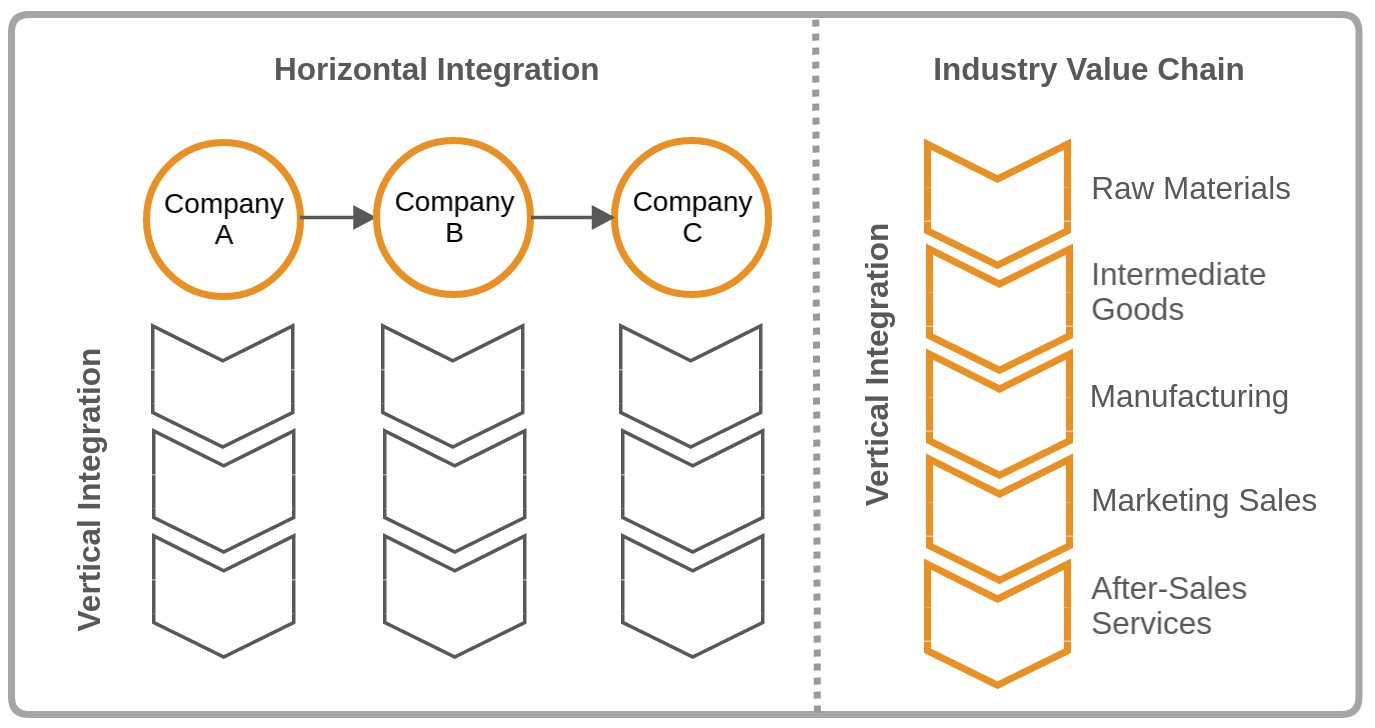
\includegraphics[width=\textwidth]{resources/images/vertical_horizontal_integration.png}
    \caption[Horizontal vs. Vertical Integration]{Horizontal vs. Vertical Integration. Adapted from: \cite{Jur2013}}
    \label{fig:vertical_horizontal_integration}
\end{figure}

Figure \ref{fig:vertical_horizontal_integration} illustrates this concept.
The left side shows the whole production process over company boundaries on the horizontal scale, as well as the industry value chain on the vertical scale which is specific for each company.
On the right side there is an exemplary industry value chain which starts with the raw materials and ends with the sale of the product to illustrates an more specific example of the vertical integration.
From a technical site this means each machine in a factory has exactly to know what they have to do.
The underlying system has to be modular and move away from a monolithic centralized system, to a decentralized system which is located locally near the machines himself.
The communication path between them have to grow shorter.
The machines have to be self organized and should communicate between each other even if the core system is not reachable because of lossy signals or other connection issues.
If this can be achieved there will be an highly flexible, individualized and resource friendly mass production, which can be cheaper, faster and can have a much higher fault tolerance.


\subsection{Cyber Physical Systems}
As we already now, in smart factories every physical device is connected to each other.
Everything can be captured and monitored in each step of a production process.
With \acp{CPS} every physical entity has a digital representation in the virtual system.\cite[cf.][p. 1363]{Poovendran:2010}
Before a \ac{CS} was passive, which means there was no communication between the physical and the virtual world.\cite[cf.][p. 1364]{Poovendran:2010}
While new technologies in the physical world, like new materials, hardware and energy, are developed, the technologies in the virtual worlds are also being improved, for example through the use of new protocols, networking, storage and computing technologies.\cite[cf.][p. 1364]{Poovendran:2010}
This adds more intelligence in such systems, as well as a much more flexible and modular structure.
A \ac{CPS} can organize production automatically and autonomously, which eliminate the need of having a central process control.\cite[cf.]{Lom:2016}
Thereby the system can handle lossy signals and short range radio technologies, which are widely used in such a context.\cite[cf.]{Yannuzzi2014}
In summary \acp{CPS} can help to enable the vision of Smart Factories in both the horizontal as well as the vertical integration.


\subsection{Fog Computing}
In the beginning of Cloud Computing most of the systems based on a monolithical architecture.
Over time the system was broken down to a more distributes multicloud architecture, similar to microservices.
With the appearance of Fog Computing the Cloud also moves from centralized data centers to the edge of the underlying network.
Main goal is to improve the efficiency, reduce the traffic and the amount of data which is transfered to the cloud and also process, analyse and store data locally, as well as keeping sensitive data inside the network for security reasons.\cite[cf.][p. 236]{Brito2016}\cite[cf.][p. 325]{Yannuzzi2014}\cite[cf.][p. 4]{Lom:2016}
In contrast to the goals the definition and understanding of Fog Computing differs.
One perspective is to that the processing of the data take place on smart devices, e.g. sensors, embedded systems, etc., at the end of the network or in smart router or other gateway devices.\cite[cf.][p. 4]{Lom:2016}
Another interpretation is that fog computing appears as an intermediate layer between smart devices and the cloud.\cite[cf.][p. 236]{Brito2016}
Processing the data near devices enables lower latency and real-time applications can take decisions based on analytics running there.
That is important because a continuous connection to the cloud can not always be ensured.
However fog computing should not be seen as a competitor of cloud computing, it is a perfect ally for use cases where cloud computing alone is not feasible.\cite[cf.][p. 325]{Yannuzzi2014}


\section{Virtualization}
According to the \ac{NIST} the definition of virtualization is: "Virtualization is the simulation of the software and/or hardware upon which other software runs. This
simulated environment is called a virtual machine (VM)."\cite{Sca2011}.
This means a \ac{VM}, also referred as guest system, can be executed in a real system, which is referred as host system.
A \ac{VM} has its own \ac{OS} which is completely isolated from the other \acp{VM} and the host system.\cite[cf.][p. 2]{Celesti:2016}
Basically there are two types of virtualization: Process virtualization where the virtualizing software also known as \ac{VMM} is executed by the host \ac{OS} and only an application will be executed inside the guest \ac{OS} and on the other side there is the the system virtualization where the whole \ac{OS} as well as the application are running inside the virtualizing software.
Figure \ref{fig:vms_vs_docker} illustrate both concepts.
Examples for process virtualization could be the \ac{JVM}\footnote{\url{https://www.java.com}}, the .Net framework\footnote{\url{https://www.microsoft.com/net}} or Docker\footnote{\url{https://www.docker.com}}, where VMWare\footnote{\url{http://www.vmware.com}}, Oracle Virtual Box\footnote{\url{https://www.virtualbox.org}}, XEN\footnote{\url{https://www.xenproject.org}} or Microsoft Hyper-V\footnote{\url{https://www.microsoft.com/de-de/cloud-platform/server-virtualization}} are only some examples for system virtualization.
The benefits of all virtualization techniques are the rapid provisioning of resources which could be \ac{RAM}, disk storage, computation power or network bandwidth.
Beside that, no human interaction is necessary during the provisioning process.
Elasticity which scales a system in a cost-efficient manner in both directions, up and down.
Customer as well as the provider profit from such a system.
Security based on the isolation of the \acp{VM} is another huge benefit.
Different processes can not interfere with each other and the data of a single user can not be accessed by other users of the same hardware.
A challenge despite all the mentioned benefits is the performance.
Running \acp{VM} increases the overhead and reduces the overall performance of a system.
Therefore the specific use case have to consider these behavior.

\begin{figure}[H]
    \centering
    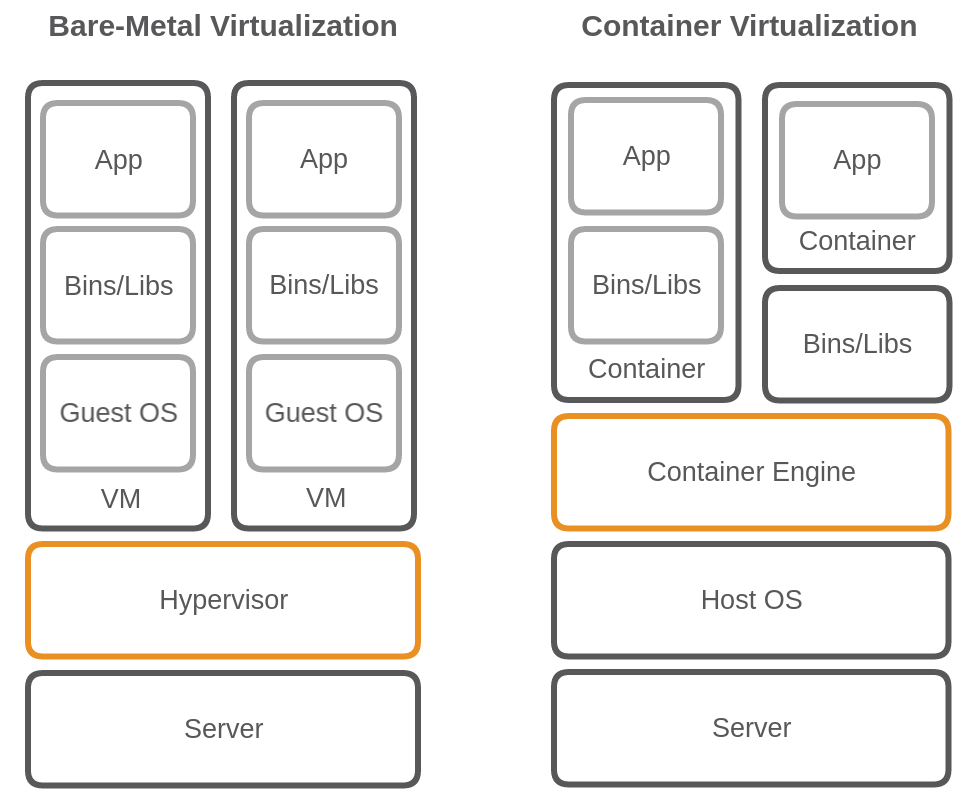
\includegraphics[width=0.6\textwidth]{resources/images/vm_vs_container.png}
    \caption[Structure bare-metal virtualization vs. container virtualization]{Structure bare-metal virtualization vs. container virtualization. Adapted from: \cite[p. 2]{Gallagher:2015}}
    \label{fig:vms_vs_docker}
\end{figure}


\subsection{Virtual Machines}
\acp{VM} are the core virtualization mechanism in cloud computing.
There are also two different designs for hardware virtualization.
The first and more popular type for cloud computing is the \textit{bare-metal virtualization}.
It needs only a basic OS to schedule \acp{VM}.
The hypervisor runs directly on the hardware of the machine without any host \ac{OS} in between.
This is more efficient, but requires special device drivers to be executed.
The other type is the \textit{hosted virtualization}.
Unlike the first type the \ac{VMM} run as a host \ac{OS} process and the \acp{VM} as a process supported by the \ac{VMM}.
No special drivers are needed for these type of virtualization, but by comparison the overhead is much bigger.
For both types, the performance limitation remains.
Each \ac{VM} need a full guest \ac{OS} image in addition to binaries and libraries which are necessary for the application to be executed.\cite[cf.][p. 381]{Pahl:2015}
If only a single application, which only needs a few binaries and libraries, is needed to be virtualized, \acp{VM} are too bloated.


\subsection{Container Virtualization}
Container virtualization which is also known as Operating System-level virtualization, is the second virtualization mechanism.
It based on fast and lightweight process virtualization to encapsulate an entire application with its dependencies into a ready-to-deploy virtual container.\cite[cf.][p. 72]{Tosatto:2015}
Such a container can be executed on the host \ac{OS} which allows an application to run as a sandboxed user-space instance.\cite[cf.][p. 1]{Anderson:2016}
All containers share a single \ac{OS} kernel, so the isolation supposed to be weaker compared to hypervisor based virtualization.\cite[cf.][p. 2]{Celesti:2016}
Compared to \acp{VM}, the number of containers on the same physical host can be much higher, because the overhead of a full \ac{OS} virtualization is eliminated.\cite[cf.][p. 2]{Celesti:2016}


\subsubsection{Linux Containers}
When we talk about container virtualization nowadays, Docker have to become one of the most famous tools out there.
It based on \ac{LXC}\footnote{\url{https://linuxcontainers.org/}} a technology which uses kernel mechanisms like \textit{namespaces} or \textit{cgroups} to isolate processes on a shared \ac{OS}.\cite[cf.][p. 381]{Pahl:2015}
Namespaces for example are used to isolate groups of processes whereas cgroups are used to manage and limit resources access just like restricting the memory, disc space or \ac{CPU} usage.\cite[cf.][p. 381]{Pahl:2015}
"The goal of \ac{LXC} is to create an environment as close as possible to a standard Linux installation but without the need for a separate kernel."\cite[p. 72]{Tosatto:2015}
There are several other container virtualization tools out there like OpenVZ\footnote{\url{https://openvz.org/Main_Page}} or Linux-VServer\footnote{\url{http://www.linux-vserver.org}}.
In contrast to them, an advantage of \ac{LXC} is that it runs on an unmodified Linux kernel.
This means that LXC can be executed in most of the popular Linux distributions these days.


\subsubsection{Docker}
As mentioned before, Docker based on \ac{LXC}.
This allows the Docker Engine to build, deploy and run containers in an easy and customizable way.
Similar to \acp{VM}, containers are executed from images.
A mayor benefit of Docker is the fact, that Docker images can be combined like build blocks.
Each image can build on top of another.
Figure \ref{fig:docker_container_structure} illustrates the concept for the image of the pretty famous Django\footnote{\url{https://www.djangoproject.com/}} web framework.
In that case, the Django image, which is the resulting image, based on the Python 3.4 image which again based on the Debian Jessy image.
All of them are read-only, but Docker adds a writeable layer, also known as \textit{container layer}, on top of the images as soon as the container will be created.
File system operations such as creating new files, modifying or deleting existing files are written directly to these layer.\cite[cf.]{dockerImages}
The other images don\'t get involved.
These chaining mechanism of images allows Docker to ease the use of dependencies and administrative overhead.

\begin{figure}[H]
    \centering
    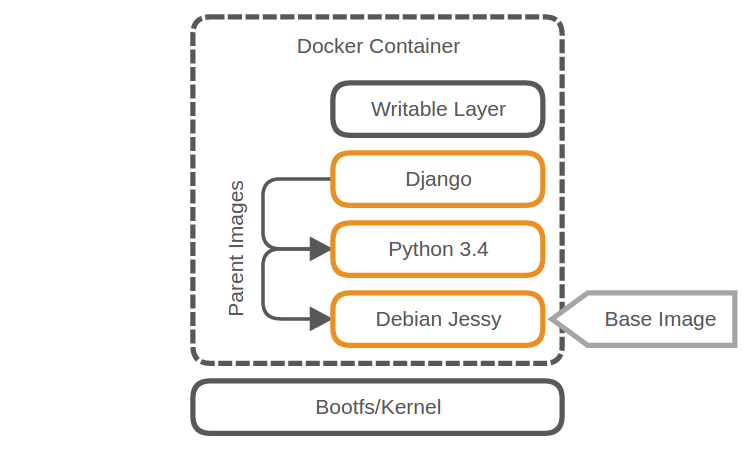
\includegraphics[width=0.75\textwidth]{resources/images/docker_container_structure.png}
    \caption[Docker container structure]{Docker container structure.}
    \label{fig:docker_container_structure}
\end{figure}

Beside that, Docker is splitted up in several components, such as the Docker Engine, the Docker Registries and Docker Compose to mention only a few.
The Docker Engine is a client-server application which can be distinguished by the Docker client, a \ac{REST} \ac{API} and the Docker server.
Latter is a daemon process which "creates and manages Docker objects, such as images, containers, networks, and data volumes"\cite{dockerEngine}.
The client is a \ac{CLI}, which interact via a \ac{REST} \ac{API} with the daemon.\cite[cf.]{dockerEngine}

% Docker Registries
Another component, the Docker Registry, is basically a library of Docker images.
They can be public or private available, as well as on the same machine like the Docker daemon or an external server.\cite[cf.]{dockerEngine}
The most popular one it the official Docker Hub\footnote{\url{https://hub.docker.com}}.
There is also an Docker Store\footnote{\url{https://store.docker.com}}, where customers can buy and sell trusted and enterprise ready containers and plugins.
With the Docker client it is pretty easy to \textit{search} for new containers and to \textit{pull} containers from or \textit{push} containers to a specific repository.

% Docker Compose
With Docker Compose multiple Docker Containers can be executed as a single application.
Therefore YAML compose file will be used to configure and combine the services.
For example the already mentioned Django image can be executed and linked together with a MongoDB\footnote{\url{https://www.mongodb.com}} images.
The main benefit is the ease of configure dependencies between several containers and configuration steps.
These concept is similar to deployment tools like Vagrant\footnote{\url{https://www.vagrantup.com}}, Ansible\footnote{\url{https://www.ansible.com}} or Puppet\footnote{\url{https://puppet.com}}.

% Benefits
A major benefit of Docker is that the execution environment of an application is completely the same on a local machine as on the production environment.\cite[cf.][p. 2]{Gallagher:2015}
There is no need to do things differently when switching from a development environment like a local machine, to a production environment like a server.\cite[cf.][p. 2]{Gallagher:2015}


\subsection{Container Orchestration}
Containers by itself helps to develop and deploy applications, but containers release their full potential only when they are used together with an orchestration engine.
Before orchestration engines, the deployment of an application or service was realized via \ac{CI} and deployment tools like Vagrant or Ansible.
Deployment scripts or plans was created and be executed every time an application changed or should be scaled up on a new machine.
This was less flexible and error-prone.
Orchestration engines cover these needs by automatically choosing new machines, deploying containers, handle the lifecycle of them and monitor the system.
These flexibility enables a new level of abstraction and automatization of deployment.
There are a bunch of orchestration engines out there.
For Docker, Kubernetes and Docker Swarm are the most popular at the moment.


\subsubsection{Kubernetes}
Kubernetes is an open source container cluster manager which was released 2014 by Google.
It is "a platform for automating deployment, scaling, and operations"\cite[p. 1]{Grant:2015} of containers.
Therefore a cluster of containers can be created and managed.
The system can for example schedule on which node a container should be executed, handle node failures, can scale the cluster by adding or removing nodes or enable rolling updates.\cite[p. 5 f.]{Grant:2015}

\begin{figure}[H]
    \centering
    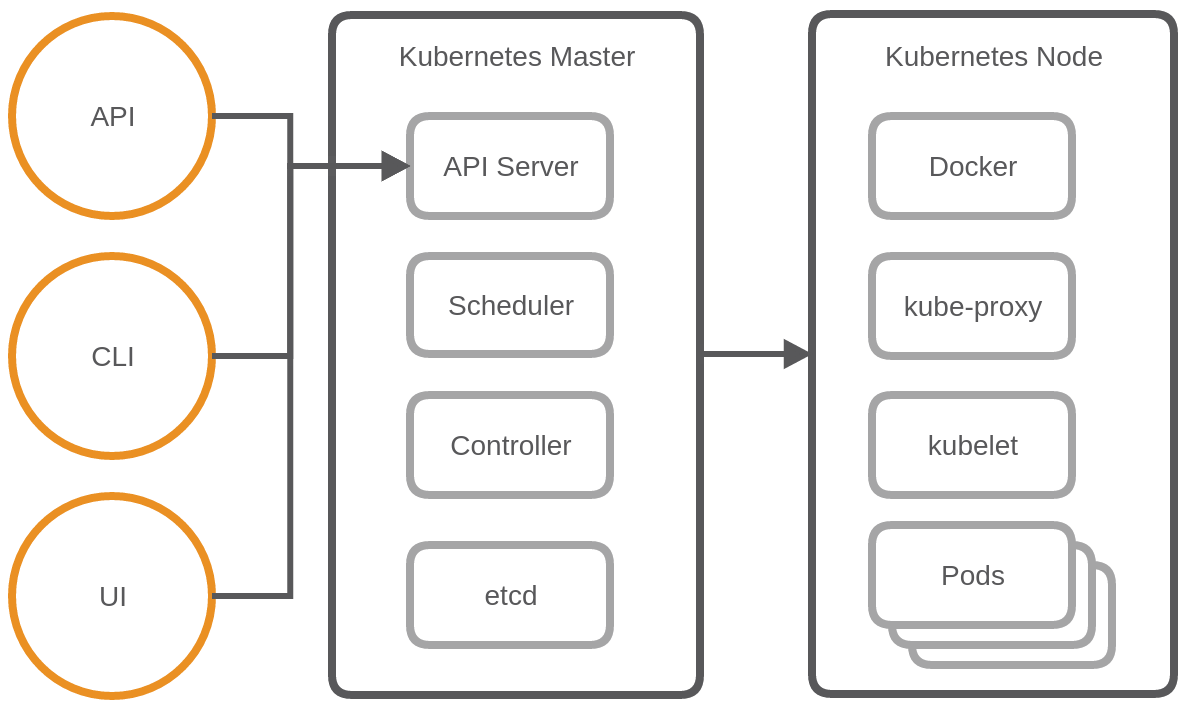
\includegraphics[width=0.75\textwidth]{resources/images/kubernetes_architecture.png}
    \caption[Kubernetes architecture]{Kubernetes architecture. Adapted from: \cite{MSV:2016}}
    \label{fig:kubernetes_architecture}
\end{figure}

Figure \ref{fig:kubernetes_architecture} illustrates the basic architecture of Kubernetes.
The user can interact with the Kubernetes system via a \ac{CLI}, an \ac{UI} or a third party application, over a \ac{REST} \ac{API} to the Kubernetes Master or more specifically the \ac{API} Server in the master.
The master himself controls the one or multiple nodes, monitor the system, schedule resources or pull new images from the repository, to name only a few tasks.
Each node has a two way communication with the master via a kubelet.
In addition each node has the services necessary to run container applications like Docker.
Furthermore Kubernetes can combine one or multiple containers into one so called Pod.\cite[cf.][p. 7]{Mulyana:2016}
"Pods are always co-located and co-scheduled, and run in a shared context."\cite{Kubernetes:pods:2016}
One node again can execute multiple Pods.
Pods are only temporary grouped containers with a non-stable IP address.
After a Pod is destroyed it can never be resurrected.
Pods can also share functionality to other Pods inside a Kubernetes cluster.
A logical set of Pods and the access policy of them is called a Kubernetes service.
Such a service can abstract multiple Pod replicas and manage them.
A frontend which have access to the service do not care about changes in the service.
Any change, be it a down scale or an up scale of the system, remains unseen for the frontend.
They are exposed through internal or external endpoints to the users or the cluster.\cite[cf.][p. 11]{MSV:2016}
Labels can be used to organize and to select subsets of Kubernetes Objects, such as Pods or Services.\cite[cf.]{Kubernetes:labels:2016}
They are simply key/value pairs which and should be meaningful and relevant to users, but do not imply semantics to the core system.\cite[cf.]{Kubernetes:labels:2016}
The kube-proxy is a network proxy and load balancer which is accessible from the outside of the system via a Kubernetes service.\cite[cf.][p. 7]{Mulyana:2016}
"Each node and can do simple TCP,UDP stream forwarding or round robin TCP,UDP forwarding across a set of backends."\cite{Kubernetes:kube-proxy:2016}
The Replication Controller is one of the mayor controllers in a Kubernetes System.
It ensures that a specified number of pod replicas are running and available at any time.\cite[cf.]{Kubernetes:replication-controller:2016}
If for example one node disappear because of connection issues, the Replication Controller will start a new one.
If the disappeared node is available back again it will kill a node.
These functionality increases the stability, the availability and the scalability of the system in an autonomous manner.
The last important component in Kubernetes are rolling updates.
With rolling updates the system can update one pod at a time, rather than taking down the entire service and update the whole system.\cite[cf.]{Kubernetes:rolling-updates:2016}
This also increases the stability and availability of the system and eases the managing of container clusters.


\subsection{Network Function Virtualization}
\ac{NFV} is an architectural framework to provide a methodology for the design, implementation, and deployment of \acp{NF} through software virtualization.\cite[cf.][p. 8]{ETSI:NFV:2013}\cite[cf.]{Rivenes:2014}
"These \acp{NF} are referred as \acp{VNF}."\cite[p. 8]{ETSI:NFV:2013}
It takes into consideration \ac{SDN} and preparing for the use of non-proprietary software to hardware integrations instead of multiple vendor specific devices for each function, e.g. routers, firewalls, storages, switches, etc.\cite[cf.]{Rivenes:2014}
Now high-performance firewalls and load balancing software for example can run on commodity PC hardware and traffic can be off-loaded onto inexpensive programmable switches.\cite[cf.]{Noble:2015}
Some benefits are speed, agility and cost reduction in deployment as well as executional manner.\cite[cf.]{Noble:2015}
Using homogeneous hardware simplifies the process of planning and reduces power, cooling and space needs.\cite[cf.]{Noble:2015}
Through virtualization providers can utilize resources more effectively, by allocating only the necessary resources for a specific functionality.\cite[cf.]{Noble:2015}
Overall \ac{NFV} can reduce \ac{OpEx} as well as \ac{CapEx} and can decreasing the time necessary to deploy new services to the network.\cite[cf.]{Noble:2015}
To achieve \ac{NFV} the \ac{ETSI} has defined a framework for \ac{MANO}\footnote{\url{http://www.etsi.org/deliver/etsi_gs/NFV-MAN/001_099/001/01.01.01_60/gs_NFV-MAN001v010101p.pdf}} of \acp{VNF}.

\section{Conclusion}
\todo{write more ---------------}
